\chapter{Strutture dati specializzate}
Finora abbiamo esaminato una serie di \emph{strutture dati} e per ciascuna
ne abbiamo anche analizzato il costo delle operazioni. È possibile però
definire \emph{strutture dati speciali}, o per meglio dire \q{\emph{specializzate}},
nelle quali vengono implementate soltanto alcune delle operazioni e per questo
motivo quelle implementazioni possono essere realizzare in modo più efficiente.

In questo capitolo vedremo due esempi di \emph{strutture specializzate}: le
\emph{code a priorità} e gli \emph{insiemi disgiunti}.

\section{Code a priorità}
\begin{definition}[Coda a priorità]
    Una coda a priorità è una struttura dati astratta, simile a una coda, in
    cui ogni elemento possiede un valore che ne indica la \q{priorità} e che
    viene usato per stabilire l'ordine di estrazione degli elementi dalla
    struttura.
\end{definition}

\noindent
Esistono due tipi di \emph{code a priorità} (\emph{priority queue}):
\begin{itemize}
    \item \emph{Min-priority queue}: l'estrazione avviene per valori crescenti
    di priorità;
    \item \emph{Max-priority queue}: l'estrazione avviene per valori decrescenti
    di priorità;
\end{itemize}

\paragraph{Specifica}
\begin{code}{MINPRIORITYQUEUE}
    \com{Crea una \emph{coda a priorità} con capacità $n$}
    \bc{PRIORITYQUEUE} PriorityQueue(\bc{int} n)
    \nl\com{Restituisce \bc{true} se la \emph{coda a priorità} è vuota}
    \bc{boolean} isEmpty()
    \nl\com{Restituisce l'elemento minimo di una \emph{coda a priorità} non vuota}
    \bc{ITEM} min()
    \nl\com{Rimuove e restituisce l’elemento minimo di una \emph{coda a priorità} non vuota}
    \bc{deleteMin()}
    \nl\com{Inserisce l'elemento $x$ con priorità $p$ nella \emph{coda a priorità} e restituisce}
    \com{un oggetto \bc{PRIORITYITEM} che identifica $x$ all'interno della \emph{coda}}
    \bc{PRIORITYITEM} insert(\bc{ITEM} x, \bc{int} p)
    \nl\com{Diminuisce la priorità dell’oggetto identificato da $y$ portandola a $p$}
    decrease(\bc{PRIORITYITEM} y, \bc{int} p)
\end{code}
\begin{note}
    La specifica di una \emph{max-priority queue} è uguale, ma invece delle
    operazioni \texttt{min}, \texttt{deleteMin} e \texttt{decrease} ha
    \texttt{max}, \texttt{deleteMax} e \texttt{increase}.
\end{note}\noindent
Utilizzando le \emph{strutture dati} viste finora possiamo calcolare i seguenti
costi:

\begin{table}[h!]
\resizebox{\linewidth}{!}{
\centering
\renewcommand{\arraystretch}{1.3}
\begin{tabular}{|c|c|c|c|c|}
    \hline
    \textbf{Operazione} & $\begin{array}[c]{c}
        \textbf{Lista}\\
        \textbf{Vettore non ordinato}
    \end{array}$ & \textbf{Lista ordinata} & \textbf{Vettore ordinato} &
    \textbf{Albero Red-Black}\\
    \hline
    \textbf{min} & $O(n)$ & $O(1)$ & $O(1)$ & $O(\log n)$\\
    \hline
    \textbf{deleteMin} & $O(n)$ & $O(1)$ & $O(n)$ & $O(\log n)$\\
    \hline
    \textbf{insert} & $O(n)$ & $O(n)$ & $O(n)$ & $O(\log n)$\\
    \hline
    \textbf{decrease} & $O(n)$ & $O(n)$ & $O(\log n)$ & $O(\log n)$\\
    \hline
\end{tabular}}
\end{table}

\noindent
È possibile fare meglio di così?

La risposta è sì, utilizzando uno \emph{heap}, una \emph{struttura dati speciale}
che associa i vantaggi di un \emph{albero}, cioè la \emph{complessità} $O(\log n)$,
e la memorizzazione efficiente ottenibile con i normali vettori.

\subsection{Heap}
La \emph{struttura dati} dello \emph{heap} fu inventata da J. Williams nel
1964 con l'obiettivo di realizzare l'algoritmo di ordinamento \emph{HeapSort}.
Vediamo come si è arrivati all'ideazione dello \emph{heap}.

\bigskip\noindent
Consideriamo un \emph{albero binario perfetto} come il seguente:
\begin{figure}[h!]
    \centering
    \begin{graph}
        \node[main] (0) {$a$};
        \node[main] (1) [below left of=0, xshift=-10, yshift=-20] {$b$};
        \node[main] (2) [below right of=0, xshift=10, yshift=-20] {$c$};
        \node[main] (3) [below left of=1, xshift=10, yshift=-20] {$d$};
        \node[main] (4) [below right of=1, xshift=-10, yshift=-20] {$e$};
        \node[main] (5) [below left of=2, xshift=10, yshift=-20] {$f$};
        \node[main] (6) [below right of=2, xshift=-10, yshift=-20] {$g$};
      
        \path[-]  (0) edge (1)
                  (0) edge (2)
                  (1) edge (3)
                  (1) edge (4)
                  (2) edge (5)
                  (2) edge (6);
    \end{graph}
    \caption{\emph{Albero binario perfetto}}
\end{figure}

\noindent
Tutte le \emph{foglie} sono alla stessa \emph{profondità} $h$ e tutti i \emph{nodi}
interni hanno \emph{grado uscente} pari a 2. Se $n$ è il numero di \emph{nodi},
l'\emph{altezza} vale $h=\lfloor\log n\rfloor$ e, data l'\emph{altezza} $h$, il
numero di \emph{nodi} è $n=2^{h+1}-1$.

\bigskip\noindent
Cosa accade se si aggiunge un \emph{nodo}?

Ovviamente l'\emph{albero} non può più essere definito \emph{perfetto}. Supponiamo
però di \q{accatastare} tutti i nuovi \emph{nodi} a partire da sinistra. In questo
modo otteniamo un \emph{albero binario completo} nel quale tutte le \emph{foglie}
hanno \emph{profondità} $h$ o $h-1$, i \emph{nodi} al \emph{livello} $h$ sono
\q{accatastati} a sinistra e tutti \emph{nodi} interni hanno \emph{grado uscente}
pari a 2 eccetto al più uno. Come prima poi, per l'\emph{altezza} $h$ vale $h=\lfloor
\log n\rfloor$.

\begin{figure}[ht]
    \centering
    \begin{graph}
        \node[main] (0) {$a$};
        \node[main] (1) [below left of=0, xshift=-10, yshift=-20] {$b$};
        \node[main] (2) [below right of=0, xshift=10, yshift=-20] {$c$};
        \node[main] (3) [below left of=1, xshift=10, yshift=-20] {$d$};
        \node[main] (4) [below right of=1, xshift=-10, yshift=-20] {$e$};
        \node[main] (5) [below left of=2, xshift=10, yshift=-20] {$f$};
      
        \path[-]  (0) edge (1)
                  (0) edge (2)
                  (1) edge (3)
                  (1) edge (4)
                  (2) edge (5);
    \end{graph}
    \caption{\emph{Albero completo}}
\end{figure}
\begin{definition}[Albero min-heap]
    Un albero min-heap è un albero binario completo tale per cui il valore
    memorizzato in ogni nodo è minore dei valori memorizzati nei suoi figli.
\end{definition}
\begin{definition}[Albero max-heap]
    Un albero max-heap è un albero binario completo tale per  cui il valore
    memorizzato in ogni nodo è maggiore dei valori memorizzati nei suoi figli.
\end{definition}

\begin{figure}[th]
    \centering
    \begin{graph}
        \node[main] (0) {$16$};
        \node[main] (1) [below left of=0, xshift=-20, yshift=-20] {$14$};
        \node[main] (2) [below right of=0, xshift=20, yshift=-20] {$10$};
        \node[main] (3) [below left of=1, xshift=0, yshift=-20] {$8$};
        \node[main] (4) [below right of=1, xshift=0, yshift=-20] {$7$};
        \node[main] (5) [below left of=2, xshift=0, yshift=-20] {$9$};
        \node[main] (6) [below right of=2, xshift=0, yshift=-20] {$3$};
        \node[main] (7) [below left of=3, xshift=20, yshift=-20] {$2$};
        \node[main] (8) [below right of=3, xshift=-20, yshift=-20] {$4$};
        \node[main] (9) [below left of=4, xshift=20, yshift=-20] {$1$};
      
        \path[-]  (0) edge (1)
                  (0) edge (2)
                  (1) edge (3)
                  (1) edge (4)
                  (2) edge (5)
                  (2) edge (6)
                  (3) edge (7)
                  (3) edge (8)
                  (4) edge (9);
    \end{graph}
    \caption{\emph{Albero max-heap}}
\end{figure}\noindent
Un \emph{albero heap} non impone un ordinamento totale tra i \emph{figli} di un
\emph{nodo}, bensì definisce un \emph{ordinamento parziale} e quindi soddisfa
le seguenti tre proprietà:
\begin{itemize}
    \item \emph{Riflessività}: ogni \emph{nodo} è maggiore o uguale a se stesso;
    \item \emph{Antisimmetria}: se $n\geq m$ e $m\geq n$, allora $m=n$;
    \item \emph{Transitività}: se $n\geq m$ e $m\geq r$, allora $n\geq r$;
\end{itemize}
\begin{note}
    Un ordinamento parziale è una nozione più debole, ma più facile da
    realizzare.
\end{note}

\paragraph{Memorizzazione}
Un \emph{albero heap} può essere rappresentato mediante un \emph{vettore heap},
cioè un vettore nel quale, se la \emph{radice} è in posizione 1, il \emph{padre}
e i \emph{figli sinistro} e \emph{destro} di un \emph{nodo} in posizione $i$ si
trovano rispettivamente alle posizioni $p(i)=\lfloor i/2\rfloor$, $l(i)=2i$ e $r(i)=2i+1$.

Se invece la \emph{radice} è in posizione 0, gli indici del \emph{padre} e dei
\emph{figli} diventano rispettivamente $p(i)=\lfloor(i-1)/2\rfloor$, $l(i)=2i+1$
e $r(i)=2i+2$.

\begin{figure}[h!]
    \centering
    \subfloat[\emph{Albero heap} con \emph{radice} in 1]
    {
        \resizebox*{0.48\textwidth}{!}{
            \begin{graph}
                \node[main, label={$A[1]$}] (0) {$16$};
                \node[main, label={$A[2]$}] (1) [below left of=0, xshift=-20, yshift=-20] {$14$};
                \node[main, label={$A[3]$}] (2) [below right of=0, xshift=20, yshift=-20] {$10$};
                \node[main, label={$A[4]$}] (3) [below left of=1, xshift=0, yshift=-20] {$8$};
                \node[main, label={$A[5]$}] (4) [below right of=1, xshift=0, yshift=-20] {$7$};
                \node[main, label={$A[6]$}] (5) [below left of=2, xshift=0, yshift=-20] {$9$};
                \node[main, label={$A[7]$}] (6) [below right of=2, xshift=0, yshift=-20] {$3$};
                \node[main, label=below:{$A[8]$}] (7) [below left of=3, xshift=20, yshift=-20] {$2$};
                \node[main, label=below:{$A[9]$}] (8) [below right of=3, xshift=-20, yshift=-20] {$4$};
                \node[main, label=below:{$A[10]$}] (9) [below left of=4, xshift=20, yshift=-20] {$1$};
              
                \path[-]  (0) edge (1)
                          (0) edge (2)
                          (1) edge (3)
                          (1) edge (4)
                          (2) edge (5)
                          (2) edge (6)
                          (3) edge (7)
                          (3) edge (8)
                          (4) edge (9);
            \end{graph}
        }
    }
    \hfill
    \subfloat[\emph{Albero heap} con \emph{radice} in 0]
    {
        \resizebox*{0.48\textwidth}{!}{
            \begin{graph}
                \node[main, label={$A[0]$}] (0) {$16$};
                \node[main, label={$A[1]$}] (1) [below left of=0, xshift=-20, yshift=-20] {$14$};
                \node[main, label={$A[2]$}] (2) [below right of=0, xshift=20, yshift=-20] {$10$};
                \node[main, label={$A[3]$}] (3) [below left of=1, xshift=0, yshift=-20] {$8$};
                \node[main, label={$A[4]$}] (4) [below right of=1, xshift=0, yshift=-20] {$7$};
                \node[main, label={$A[5]$}] (5) [below left of=2, xshift=0, yshift=-20] {$9$};
                \node[main, label={$A[6]$}] (6) [below right of=2, xshift=0, yshift=-20] {$3$};
                \node[main, label=below:{$A[7]$}] (7) [below left of=3, xshift=20, yshift=-20] {$2$};
                \node[main, label=below:{$A[8]$}] (8) [below right of=3, xshift=-20, yshift=-20] {$4$};
                \node[main, label=below:{$A[9]$}] (9) [below left of=4, xshift=20, yshift=-20] {$1$};
              
                \path[-]  (0) edge (1)
                          (0) edge (2)
                          (1) edge (3)
                          (1) edge (4)
                          (2) edge (5)
                          (2) edge (6)
                          (3) edge (7)
                          (3) edge (8)
                          (4) edge (9);
            \end{graph}
        }
    }\\
    \subfloat[\emph{Vettore heap} con \emph{radice} in 1]
    {
        \resizebox*{0.48\textwidth}{!}{
            \begin{graph}
                \node[rectangle, draw, label={$A[1]$}, minimum width=10mm, minimum height=10mm]
                    (0) {\texttt{16}};
                \node[rectangle, draw, label={$A[2]$}, minimum width=10mm, minimum height=10mm]
                    (1) [right of=0, xshift=-28.5] {\texttt{14}};
                \node[rectangle, draw, label={$A[3]$}, minimum width=10mm, minimum height=10mm]
                    (2) [right of=1, xshift=-28.5] {\texttt{10}};
                \node[rectangle, draw, label={$A[4]$}, minimum width=10mm, minimum height=10mm]
                    (3) [right of=2, xshift=-28.5] {\texttt{8}};
                \node[rectangle, draw, label={$A[5]$}, minimum width=10mm, minimum height=10mm]
                    (4) [right of=3, xshift=-28.5] {\texttt{7}};
                \node[rectangle, draw, label={$A[6]$}, minimum width=10mm, minimum height=10mm]
                    (5) [right of=4, xshift=-28.5] {\texttt{9}};
                \node[rectangle, draw, label={$A[7]$}, minimum width=10mm, minimum height=10mm]
                    (6) [right of=5, xshift=-28.5] {\texttt{3}};
                \node[rectangle, draw, label={$A[8]$}, minimum width=10mm, minimum height=10mm]
                    (7) [right of=6, xshift=-28.5] {\texttt{2}};
                \node[rectangle, draw, label={$A[9]$}, minimum width=10mm, minimum height=10mm]
                    (8) [right of=7, xshift=-28.5] {\texttt{4}};
                \node[rectangle, draw, label={$A[10]$}, minimum width=10mm, minimum height=10mm]
                    (9) [right of=8,xshift=-28.5] {\texttt{1}};
            \end{graph}
        }
    }
    \hfill
    \subfloat[\emph{Vettore heap} con \emph{radice} in 0]
    {
        \resizebox*{0.48\textwidth}{!}{
            \begin{graph}
                \node[rectangle, draw, label={$A[0]$}, minimum width=10mm, minimum height=10mm]
                    (0) {\texttt{16}};
                \node[rectangle, draw, label={$A[1]$}, minimum width=10mm, minimum height=10mm]
                    (1) [right of=0, xshift=-28.5] {\texttt{14}};
                \node[rectangle, draw, label={$A[2]$}, minimum width=10mm, minimum height=10mm]
                    (2) [right of=1, xshift=-28.5] {\texttt{10}};
                \node[rectangle, draw, label={$A[3]$}, minimum width=10mm, minimum height=10mm]
                    (3) [right of=2, xshift=-28.5] {\texttt{8}};
                \node[rectangle, draw, label={$A[4]$}, minimum width=10mm, minimum height=10mm]
                    (4) [right of=3, xshift=-28.5] {\texttt{7}};
                \node[rectangle, draw, label={$A[5]$}, minimum width=10mm, minimum height=10mm]
                    (5) [right of=4, xshift=-28.5] {\texttt{9}};
                \node[rectangle, draw, label={$A[6]$}, minimum width=10mm, minimum height=10mm]
                    (6) [right of=5, xshift=-28.5] {\texttt{3}};
                \node[rectangle, draw, label={$A[7]$}, minimum width=10mm, minimum height=10mm]
                    (7) [right of=6, xshift=-28.5] {\texttt{2}};
                \node[rectangle, draw, label={$A[8]$}, minimum width=10mm, minimum height=10mm]
                    (8) [right of=7, xshift=-28.5] {\texttt{4}};
                \node[rectangle, draw, label={$A[9]$}, minimum width=10mm, minimum height=10mm]
                    (9) [right of=8,xshift=-28.5] {\texttt{1}};
            \end{graph}
        }
    }
    \caption{Memorizzazione \emph{alberi heap}}
\end{figure}

\noindent
Dalle definizioni di \emph{alberi min-heap} e \emph{max-heap} possiamo dedurre
delle proprietà sui relativi \emph{vettori}:
\begin{itemize}
    \item \emph{Vettori min-heap}: $A[i]\leq A[l(i)]$ e $A[i]\leq A[r(i)]$;
    \item \emph{Vettori max-heap}: $A[i]\geq A[l(i)]$ e $A[i]\geq A[r(i)]$;
\end{itemize}

\subsection{Algoritmo HeapSort}
Vediamo quindi l'algoritmo \emph{HeapSort} per l'ordinamento in senso crescente
di un vettore.

L'algoritmo ordina un vettore \q{in-place}, costruendo prima su di esso un
\emph{albero max-heap} e poi spostando progressivamente in fondo gli elementi massimi.
Ad ogni spostamento vengono ripristinate le proprietà degli \emph{alberi max-heap}.

Le funzioni utilizzate sono due:
\begin{itemize}
    \item \texttt{heapBuild}: costruisce un \emph{albero max-heap} a partire da
    un vettore non ordinato;
    \item \texttt{maxHeapRestore}: ripristina le proprietà degli \emph{alberi
    max-heap};
\end{itemize}
\begin{note}
    Tutte le operazioni vengono effettuate \q{in-place}, cioè agiscono sul vettore
    stesso senza usare \emph{strutture ausiliarie}. Quindi, l'\emph{albero max-heap}
    non viene realmente creato, ma grazie alle sue proprietà di memorizzazione,
    il vettore di input viene semplicemente interpretato come fosse un \emph{albero
    max-heap}.
\end{note}
Per questo motivo, la funzione \emph{maxHeapRestore} riceve in input un vettore $A$
e un indice $i$ e si occupa di garantire che al termine dell'esecuzione,
l'\emph{albero binario} con radice $i$ sia un \emph{albero max-heap}.

\begin{eg}[Esempio di esecuzione della maxHeapRestore]
    Consideriamo il seguente vettore:
    \[(3,\,14,\,10,\,8,\,7,\,9,\,5,\,2,\,4,\,1)\]
    e ipotizziamo di invocare \texttt{maxHeapRestore} su di esso usando come
    radice la posizione $1$.

    \begin{figure}[h!]
        \centering
        \subfloat[Situazione iniziale]
        {
            \resizebox*{0.48\textwidth}{!}{
                \begin{graph}
                    \node[main, fill=leaf, line width=1.3pt] (0) {$3$};
                    \node[main] (1) [below left of=0, xshift=-20, yshift=-20] {$14$};
                    \node[main] (2) [below right of=0, xshift=20, yshift=-20] {$10$};
                    \node[main] (3) [below left of=1, xshift=0, yshift=-20] {$8$};
                    \node[main] (4) [below right of=1, xshift=0, yshift=-20] {$7$};
                    \node[main] (5) [below left of=2, xshift=0, yshift=-20] {$9$};
                    \node[main] (6) [below right of=2, xshift=0, yshift=-20] {$5$};
                    \node[main] (7) [below left of=3, xshift=20, yshift=-20] {$2$};
                    \node[main] (8) [below right of=3, xshift=-20, yshift=-20] {$4$};
                    \node[main] (9) [below left of=4, xshift=20, yshift=-20] {$1$};
                  
                    \path[-]  (0) edge (1)
                              (0) edge (2)
                              (1) edge (3)
                              (1) edge (4)
                              (2) edge (5)
                              (2) edge (6)
                              (3) edge (7)
                              (3) edge (8)
                              (4) edge (9);
                \end{graph}
            }
        }
        \hfill
        \subfloat[Il 3 viene scambiato con il 14]
        {
            \resizebox*{0.48\textwidth}{!}{
                \begin{graph}
                    \node[main] (0) {$14$};
                    \node[main, fill=leaf, line width=1.3pt] (1) [below left of=0, xshift=-20, yshift=-20] {$3$};
                    \node[main] (2) [below right of=0, xshift=20, yshift=-20] {$10$};
                    \node[main] (3) [below left of=1, xshift=0, yshift=-20] {$8$};
                    \node[main] (4) [below right of=1, xshift=0, yshift=-20] {$7$};
                    \node[main] (5) [below left of=2, xshift=0, yshift=-20] {$9$};
                    \node[main] (6) [below right of=2, xshift=0, yshift=-20] {$5$};
                    \node[main] (7) [below left of=3, xshift=20, yshift=-20] {$2$};
                    \node[main] (8) [below right of=3, xshift=-20, yshift=-20] {$4$};
                    \node[main] (9) [below left of=4, xshift=20, yshift=-20] {$1$};
                  
                    \path[-]  (0) edge (1)
                              (0) edge (2)
                              (1) edge (3)
                              (1) edge (4)
                              (2) edge (5)
                              (2) edge (6)
                              (3) edge (7)
                              (3) edge (8)
                              (4) edge (9);

                    \path[->, dashed]   (0) edge[bend left=30] (1)
                                        (1) edge[bend left=30] (0);
                \end{graph}
            }
        }\\
        \subfloat[Il 3 viene scambiato con l'8]
        {
            \resizebox*{0.48\textwidth}{!}{
                \begin{graph}
                    \node[main] (0) {$14$};
                    \node[main] (1) [below left of=0, xshift=-20, yshift=-20] {$8$};
                    \node[main] (2) [below right of=0, xshift=20, yshift=-20] {$10$};
                    \node[main, fill=leaf, line width=1.3pt] (3) [below left of=1, xshift=0, yshift=-20] {$3$};
                    \node[main] (4) [below right of=1, xshift=0, yshift=-20] {$7$};
                    \node[main] (5) [below left of=2, xshift=0, yshift=-20] {$9$};
                    \node[main] (6) [below right of=2, xshift=0, yshift=-20] {$5$};
                    \node[main] (7) [below left of=3, xshift=20, yshift=-20] {$2$};
                    \node[main] (8) [below right of=3, xshift=-20, yshift=-20] {$4$};
                    \node[main] (9) [below left of=4, xshift=20, yshift=-20] {$1$};
                  
                    \path[-]  (0) edge (1)
                              (0) edge (2)
                              (1) edge (3)
                              (1) edge (4)
                              (2) edge (5)
                              (2) edge (6)
                              (3) edge (7)
                              (3) edge (8)
                              (4) edge (9);

                    \path[->, dashed]   (1) edge[bend left=30] (3)
                                        (3) edge[bend left=30] (1);
                \end{graph}
            }
        }
        \hfill
        \subfloat[Il 3 viene scambiato con il 4]
        {
            \resizebox*{0.48\textwidth}{!}{
                \begin{graph}
                    \node[main] (0) {$14$};
                    \node[main] (1) [below left of=0, xshift=-20, yshift=-20] {$8$};
                    \node[main] (2) [below right of=0, xshift=20, yshift=-20] {$10$};
                    \node[main] (3) [below left of=1, xshift=0, yshift=-20] {$4$};
                    \node[main] (4) [below right of=1, xshift=0, yshift=-20] {$7$};
                    \node[main] (5) [below left of=2, xshift=0, yshift=-20] {$9$};
                    \node[main] (6) [below right of=2, xshift=0, yshift=-20] {$5$};
                    \node[main] (7) [below left of=3, xshift=20, yshift=-20] {$2$};
                    \node[main, fill=leaf, line width=1.3pt] (8) [below right of=3, xshift=-20, yshift=-20] {$3$};
                    \node[main] (9) [below left of=4, xshift=20, yshift=-20] {$1$};
                  
                    \path[-]  (0) edge (1)
                              (0) edge (2)
                              (1) edge (3)
                              (1) edge (4)
                              (2) edge (5)
                              (2) edge (6)
                              (3) edge (7)
                              (3) edge (8)
                              (4) edge (9);
                  
                    \path[->, dashed]   (3) edge[bend left=30] (8)
                                        (8) edge[bend left=30] (3);
                \end{graph}
            }
        }
    \end{figure}\noindent
    Al termine dell'esecuzione abbiamo ottenuto un albero max-heap corretto.
\end{eg}

\newpage
\paragraph{Implementazione}
\begin{minicode}{Implementazione maxHeapRestore}
    \ind maxHeapRestore(\bc{ITEM}[] A, \bc{int} i, \bc{int} dim)\\
        \bc{int} max = i\hfill\com{Sceglie la \emph{radice}}
        \indf if (l(i) $\leq$ and dim A[l(i)] > A[max]) then\\
            max = l(i)\\
        \indf if (r(i) $\leq$ and dim A[r(i)] > A[max]) then\\
            max = r(i)\\
        \indf if (i $\neq$ max) then\hfill\com{Se $i == max$ l'\emph{albero} è apposto}
            swap(A, i, max)\hfill\com{Scambia la \emph{radice} e il maggiore tra i suoi \emph{figli}}
            maxHeapRestore(A, max, dim)\hfill\com{Controlla il \emph{sottoalbero} con \emph{radice} $max$}
\end{minicode}
\paragraph{Complessità}
Ad ogni chiamata vengono eseguiti $O(1)$ confronti e se il \emph{nodo} $i$ non è
massimo, si invoca ricorsivamente \texttt{maxHeapRestore} su uno dei \emph{figli}.
L'esecuzione nel caso peggiore termina al raggiungimento di una \emph{foglia},
quindi il costo è limitato dall'\emph{altezza} dell'\emph{albero}, ovvero
$T(n)=O(\log n)$.

\paragraph{Dimostrazione di correttezza}
\begin{proof}[Dimostrazione]
    Dobbiamo dimostrare che al termine dell'esecuzione l'\emph{albero} con
    \emph{radice} in $A[i]$ rispetta le proprietà degli \emph{alberi max-heap}.
    Procediamo per induzione sull'\emph{altezza} $h$ dell'\emph{albero}.

    \paragraph{Caso base} $h=0$. L'\emph{albero} è composto da un solo
    \emph{nodo} e quindi rispetta per forza le proprietà.
    \paragraph{Passo induttivo} Ipotizziamo che l'algoritmo funzioni correttamente
    su tutti gli \emph{alberi} di \emph{altezza} minore di $h$. A questo punto si
    configurano tre casi:
    \begin{itemize}
        \item \emph{Caso 1}: $A[i]\geq A[l(i)]$ e $A[i]\geq A[r(i)]$, ovvero
        il \emph{nodo} $A[i]$ è più grande dei propri \emph{figli} e quindi
        l'\emph{albero radicato} in $A[i]$ è un \emph{albero max-heap} e l'algoritmo
        termina;
        \item \emph{Caso 2}: $A[i]<A[l(i)]$ e $A[r(i)]<A[l(i)]$, ovvero il \emph{figlio
        sinistro} è più grande sia del \emph{padre} che del \emph{fratello}. Quindi,
        vengono scambiati di posizione il \emph{figlio sinistro} e il \emph{padre}.
        A questo punto valgono $A[i]\geq A[l(i)]$ e $A[i]\geq A[r(i)]$, ma il
        \emph{sottoalbero} con \emph{radice} in $A[l(i)]$ potrebbe non rispettare
        più le proprietà per gli \emph{alberi max-heap}. Di conseguenza, l'algoritmo
        continua applicando ricorsivamente \texttt{maxHeapRestore} sull'\emph{albero}
        con \emph{radice} in $A[l(i)]$, ma siccome quell'\emph{albero} ha \emph{altezza}
        minore di $h$, per ipotesi induttiva, l'algoritmo riesce correttamente a
        garantire il rispetto di tutte le proprietà;
        \item \emph{Caso 3}: $A[i]<A[r(i)]$ e $A[l(i)]<A[r(i)]$, ovvero il \emph{figlio
        destro} è più grande sia del \emph{padre} che del \emph{fratello}. Quindi,
        vengono scambiati di posizione il \emph{figlio destro} e il \emph{padre}.
        A questo punto valgono $A[i]\geq A[l(i)]$ e $A[i]\geq A[r(i)]$, ma il
        \emph{sottoalbero} con \emph{radice} in $A[r(i)]$ potrebbe non rispettare
        più le proprietà per gli \emph{alberi max-heap}. Di conseguenza, l'algoritmo
        continua applicando ricorsivamente \texttt{maxHeapRestore} sull'\emph{albero}
        con \emph{radice} in $A[r(i)]$, ma siccome quell'\emph{albero} ha \emph{altezza}
        minore di $h$, per ipotesi induttiva, l'algoritmo riesce correttamente a
        garantire il rispetto di tutte le proprietà;
    \end{itemize}
\end{proof}\noindent
Consideriamo ora la funzione \texttt{heapBuild}. La funzione riceve in input un
vettore da ordinare e, per le proprietà di memorizzazione degli \emph{alberi heap},
sappiamo che tutti i \emph{nodi} con indici compresi tra $\lfloor n/2\rfloor+1$
e $n$ sono \emph{foglie}, ovvero \emph{alberi heap} contenenti un solo elemento.

La funzione \texttt{heapBuild} quindi, non fa altro che applicare \texttt{maxHeapRestore}
a tutti i \emph{nodi}, partendo dal primo che non è una \emph{foglia}, cioè da
$A[\lfloor n/2\rfloor]$, e risalendo fino alla \emph{radice}.

\paragraph{Implementazione}
\begin{minicode}{Implementazione heapBuild}
    \ind heapBuild(\bc{ITEM}[] A, \bc{int} n)\\
        \indf for (i = $\lfloor$n/2$\rfloor$ downto 1) do\\
            maxHeapRestore(A, i, n)
\end{minicode}
\begin{figure}[h!]
    \centering
    \begin{graph}
        \node[main, label={$A[1]$}] (0) {$14$};
        \node[main, label={$A[2]$}] (1) [below left of=0, xshift=-20, yshift=-20] {$45$};
        \node[main, label={$A[3]$}] (2) [below right of=0, xshift=20, yshift=-20] {$28$};
        \node[main, label={$A[4]$}] (3) [below left of=1, xshift=0, yshift=-20] {$34$};
        \node[main, label={$A[5]$}] (4) [below right of=1, xshift=0, yshift=-20] {$15$};
        \node[main, fill=leaf, label={$A[6]$}] (5) [below left of=2, xshift=0, yshift=-20] {$20$};
        \node[main, fill=leaf, label={$A[7]$}] (6) [below right of=2, xshift=0, yshift=-20] {$22$};
        \node[main, fill=leaf, label=below:{$A[8]$}] (7) [below left of=3, xshift=20, yshift=-20] {$30$};
        \node[main, fill=leaf, label=below:{$A[9]$}] (8) [below right of=3, xshift=-20, yshift=-20] {$21$};
        \node[main, fill=leaf, label=below:{$A[10]$}] (9) [below left of=4, xshift=20, yshift=-20] {$25$};
        \node[main, fill=leaf, label=below:{$A[11]$}] (10) [below right of=4, xshift=-20, yshift=-20] {$16$};
      
        \path[-]  (0) edge (1)
                  (0) edge (2)
                  (1) edge (3)
                  (1) edge (4)
                  (2) edge (5)
                  (2) edge (6)
                  (3) edge (7)
                  (3) edge (8)
                  (4) edge (9)
                  (4) edge (10);
    \end{graph}
    \caption{\texttt{maxHeapRestore} viene applicata solo ai \emph{nodi} interni}
\end{figure}
\paragraph{Dimostrazione di correttezza}
\begin{proof}[Dimostrazione]
    Dimostriamo la seguente \emph{invariante di ciclo}:
    
    \smallskip\noindent {\em All'inizio di ogni iterazione del ciclo \texttt{for},
    i nodi $[i+1\dots n]$ sono radici di alberi heap.}
    \paragraph{Inizializzazione}
    All'inizio $i=\lfloor n/2\rfloor$. Supponiamo che $\lfloor n/2\rfloor+1$ non
    sia una \emph{foglia} e che quindi abbia almeno il \emph{figlio sinistro}.
    Se così fosse, il \emph{figlio} dovrebbe trovarsi alla posizione $2(\lfloor
    n/2\rfloor+1)=2\lfloor n/2\rfloor+2$, ma ciò sarebbe assurdo perché le posizioni
    $n+1$ e $n+2$ eccedono la dimensione massima $n$. La stessa dimostrazione
    vale anche per tutti gli indici successivi.
    \paragraph{Conservazione}
    È possibile applicare \texttt{maxHeapRestore} a ogni \emph{nodo} $i$ perché
    entrambi i \emph{nodi} alle posizioni $2i<2i+1\leq n$ sono \emph{radici}
    di \emph{alberi heap}. Al termine di ogni iterazioni, i \emph{nodi}
    $[i\dots n]$ sono \emph{radici} di \emph{alberi heap}.
    \paragraph{Conclusione} Al termine, $i=0$ e quindi il \emph{nodo} $1$ è
    \emph{radice} di un \emph{albero heap}.
\end{proof}
\paragraph{Complessità}
Sicuramente possiamo dire che \texttt{heapBuild} è un $O(n\log n)$ in quanto il costo
di \texttt{maxHeapRestore} è $O(\log n)$ e viene invocata $\lfloor n/2\rfloor=O(n)$
volte. Ma è veramente questo il costo?

\bigskip\noindent
In realtà, le operazioni \texttt{maxHeapRestore} vengono eseguite un
numero decrescente di volte in un \emph{albero} di \emph{altezza} crescente. E in
particolare, vale la seguente tabella:

\begin{table}[h!]
    \centering
    \renewcommand{\arraystretch}{1.2}
    \begin{tabular}{|c|c|}
        \hline
        \textbf{Altezza} & \textbf{\# esecuzioni}\\
        \hline
        0 & $\lfloor n/2^1\rfloor$\\
        \hline
        1 & $\lfloor n/2^2\rfloor$\\
        \hline
        2 & $\lfloor n/2^3\rfloor$\\
        \hline
        \dots & \dots\\
        \hline
        $h$ & $\lfloor n/2^{h+1}\rfloor$\\
        \hline
    \end{tabular}
\end{table}\noindent
Se questo è vero, possiamo scrivere la \emph{funzione di ricorrenza} come:
\[T(n)\begin{array}[t]{cll}
    \leq & \sum_{h=1}^{\lfloor n/2\rfloor}\frac{n}{2^{h+1}}h\\
    = & n\sum_{h=1}^{\lfloor n/2\rfloor}\left(\frac{1}{2}\right)^{h+1}h\\
    = & \frac{n}{2}\sum_{h=1}^{\lfloor n/2\rfloor}\left(\frac{1}{2}\right)^{h}h\\
    \leq & \frac{n}{2}\sum_{h=1}^{+\infty}\left(\frac{1}{2}\right)^{h}h & \quad\emph{Estensione ad infinito della somamtoria}\\
    = & \frac{n}{2}\frac{\frac{1}{2}}{\left(1-\frac{1}{2}\right)^2} & \quad\hyperlink{ser:5}{\emph{Serie geometrica infinita decrescente}}\\
    = & \frac{n}{2}\frac{\frac{1}{2}}{\left(\frac{1}{2}\right)^2}\\
    = & \frac{n}{2}2\\
    = & n = O(n)
\end{array}\]

\paragraph{Implementazione}
\begin{minicode}{Implementazione dell'algoritmo HeapSort}
    \ind heapsort(\bc{ITEM}[] A, \bc{int} n)\\
        heapBuild(A, n)\\
        \indf for (i = n downto 2) do\\
            swap(A, 1, i)\hfill\com{L'elemento massimo viene spostato in fondo}
            maxHeapRestore(A, 1, i - 1)\hfill\com{Ripristina le proprietà}
\end{minicode}\noindent
In pratica, l'\emph{HeapSort} inizia costruendo un \emph{albero max-heap} sul
vettore da ordinare. Ad ogni ciclo il primo elemento sarà sicuramente il
massimo e quindi viene scambiato di posto con l'elemento in posizione $i$.
Dopo ogni scambio viene invocata \texttt{maxHeapRestore} per ripristinare le
proprietà degli \emph{alberi max-heap}. Il tutto viene ripetuto fino a quando
$i$ non diventa 1.

\paragraph{Complessità}
La funzione \texttt{heapBuild} costa $\Theta(n)$, mentre le \texttt{maxHeapRestore}
ha un costo $\Theta(\log i)$ per $i$ che varia da $n$ a 2. La \emph{funzione di
ricorrenza} è la seguente:
\[T(n)=\sum_{i=n}^2\log i+\Theta(n)=\Theta(n\log n)\]

\paragraph{Dimostrazione di correttezza}
\begin{proof}[Dimostrazione]
    Dimostriamo la seguente \emph{invariante di ciclo}:
    
    \smallskip\noindent{\em All'inizio di ogni passo $i$ il sottovettore
    $A[i+1\dots n]$ è ordinato e ogni elemento in $A[1\dots i]$ è minore o
    al più uguale a ogni elemento in $A[i+1\dots n]$. Inoltre, l'elemento $A[1]$
    è la radice di un albero heap di dimensione $i$.}
    \paragraph{Inizializzazione}
    Dopo la \texttt{heapBuild} il primo elemento è la \emph{radice} di un
    \emph{albero max-heap} e quindi è maggiore dei propri \emph{figli} e, per la
    proprietà transitiva, anche dei \emph{figli} dei \emph{figli} fino alle
    \emph{foglie}. Alla prima iterazione quindi, $A[1]$ è il massimo e viene
    scambiato di posto con $A[i]=A[n]$. A quel punto, $A[n]$ è l'elemento
    massimo e il sottovettore $A[1\dots n-1]$ viene riorganizzato secondo le
    regole della \texttt{maxHeapRestore} portandone il massimo in $A[1]$.
    \paragraph{Conservazione}
    Per ogni $i\in[2\dots n]$, il sottovettore $A[i+1\dots n]$ è ordinato
    in senso crescente e in posizione $A[1]$ si trova l'elemento massimo del
    sottovettore $A[1\dots i]$. Al termine dell'iterazione, $A[i\dots n]$ è
    ordinato e $A[1]$ è il massimo in $A[1\dots i-1]$.
    \paragraph{Conclusione}
    Al termine, $i=1$ e quindi il sottovettore $A[2\dots n]$ è ordinato. Poiché
    vale sicuramente $A[1]\leq A[2]$, possiamo dire che tutto il vettore $A[1\dots
    n]$ è ordinato in senso crescente.
\end{proof}

\subsection{Implementazione di code a priorità}
Prima di vedere l'implementazione di una \emph{coda a priorità}, vediamo la
definizione di un \texttt{\bc{PRIORITYITEM}} e l'implementazione della funzione
\texttt{swap}.
\begin{minicode}{PRIORITYITEM}
    \bc{int} priority\hfill\com{Valore di priorità}
    \bc{ITEM} value\hfill\com{Valore}
    \bc{int} pos\hfill\com{Posizione nel vettore}
\end{minicode}
\begin{minicode}{Implementazione funzione swap}
    \ind swap(\bc{PRIORITYITEM} H, \bc{int} i, \bc{int} j)\\
        \bc{PRIORITYITEM} temp = H[i]\\
        H[i] = H[j]\\
        H[j] = temp\\
        H[i].pos = i\\
        H[j].pos = j
\end{minicode}\noindent
Di seguito quindi, vediamo l'implementazione di una \emph{min-priority queue}
come vettore di coppie $\langle valore,\,\emph{priorità}\rangle$. Ovviamente,
tutto ciò che vedremo vale simmetrico per le \emph{max-priority queue}.
\begin{minicode}{{Min-priority queue}}
    \bc{int} capacity\hfill\com{Dimensione massima della \emph{coda}}
    \bc{int} dim\hfill\com{Numero di elementi attualmente presenti nella \emph{coda}}
    \bc{PRIORITYQUEUE}[] H\hfill\com{\emph{Vettore heap}}
\end{minicode}
\newpage
\begin{codecont}
    \ind\bc{PRIORITYQUEUE} PriorityQueue(\bc{int} n)\\
        \bc{PRIORITYQUEUE} t = new \bc{PRIORITYQUEUE}\\
        t.capacity = n\\
        t.dim = 0\\
        t.H = new \bc{PRIORITYITEM}[1\dots n]\\
        return t\\

    \ind\bc{PRIORITYITEM} insert(\bc{ITEM} x, \bc{int} p)\\
        precondition: dim < capacity\\
        dim = dim + 1\\
        H[dim] = new \bc{PRIORITYITEM}\hfill\com{Aggiunge l'elemento in fondo}
        H[dim].value = x\\
        H[dim].priority = p\\
        H[dim].pos = dim\\
        \bc{int} i = dim\\
        \indf while (i > 1 and H[i].priority < H[p(i)].priority) do\\
            \indff swap(H, i, p(i))\hfill\com{Sposta il nuovo elemento nella posizione giusta}
            \indff i = p(i)\\
        \indf return H[i]\\

    \ind minHeapRestore(\bc{PRIORITYITEM}[] A, \bc{int} i, \bc{int} n)\\
        \bc{int} min = i\\
        if (l(i) $\leq$ dim and A[l(i)].priority < A[min].priority) then\\
            \indf min = l(i)\\
        \ind if (r(i) $\leq$ dim and A[r(i)].priority < A[min].priority) then\\
            \indf min = r(i)\\
        \ind if (i $\neq$ min) then\\
            \indf swap(A, i, min)\\
            \indf minHeapRestore(A, min, dim)\\

    \ind\bc{ITEM} deleteMin()\\
        precondition: dim > 0\\
        swap(H, 1, dim)\hfill\com{Scambia il primo e l'ultimo elemento}
        dim = dim - 1\\
        minHeapRestore(H, 1, dim)\hfill\com{Ripristina le proprietà}
        return H[dim + 1].value\hfill\com{Restituisce il valore dell'elemento rimosso}

    \ind\bc{ITEM} min()\\
        precondition: dim > 0\\
        return H[1].value\\
    
    \ind decrease(\bc{PRIORITYITEM} x, \bc{int} p)\\
        precondition: p < x.priority\\
        x.priority = p\\
        \bc{int} i = x.pos\\
        while (i > 1 and H[i].priority < H[p(i)].priority) do\\
            \indf swap(H, i, p(i))\hfill\com{Sposta l'elemento modificato nella posizione giusta}
            \indf i = p(i)
\end{codecont}
\paragraph{Complessità}
Tutte le operazioni che modificano gli \emph{heap} ne ripristinano anche le
proprietà. In particolare, questo viene fatto nel \emph{cammino radice-foglia}
dalla \texttt{deleteMin} e in quello \emph{nodo-radice} dalla \texttt{insert}
e dalla \texttt{decrease}. Poiché l'\emph{altezza} è $\lfloor\log n\rfloor$, il
costo di tali operazioni è $O(\log n)$.

\bigskip\noindent
La \emph{complessità} di tutte le operazioni è riassunta dalla seguente tabella:
\begin{table}[h!]
    \centering
    \renewcommand{\arraystretch}{1.2}
    \begin{tabular}{|c|c|}
        \hline
        \textbf{Operazione} & \textbf{Costo}\\
        \hline
        \texttt{insert} & $O(\log n)$\\
        \hline
        \texttt{deleteMin} & $O(\log n)$\\
        \hline
        \texttt{min} & $\Theta(1)$\\
        \hline
        \texttt{decrease} & $O(\log n)$\\
        \hline
    \end{tabular}
\end{table}

\section{Insiemi disgiunti}
In alcune applicazioni (e.g. ricerca delle \emph{componenti connesse} di un
\emph{grafo}) siamo interessati a gestire una collezione $S=\{S_1,\dots,
S_n\}$ di \emph{insiemi dinamici disgiunti}, ovvero tali per cui:
\[S_i\cap S_j=\emptyset\quad\forall i,j : i\neq j\]
\[\bigcup_{1=1}^n S_i=S\quad\text{con}\ n=\left|S\right|\]
Definiamo quindi un \emph{merge-find set} come una struttura dati con le
seguenti primitive:
\begin{itemize}
    \item Creazione di $n$ \emph{insiemi disgiunti} composti da un elemento
    ciascuno;
    \item \texttt{find}: identificazione dell'\emph{insieme} a cui appartiene un
    elemento;
    \item \texttt{merge}: unione di due \emph{insiemi};
\end{itemize}\noindent
Ogni insieme è identificato da un proprio elemento che viene designato come
\emph{rappresentante}. Di conseguenza, la primitiva \texttt{find} deve restituire
il \emph{rappresentante} dell'\emph{insieme} in cui si trova elemento cercato.
Definito l'elemento \emph{rappresentante}, questo può essere cambiato solo in
caso di unione con un altro \emph{insieme}.

\begin{note}
    Per semplicità di esposizione, ipotizziamo che gli elementi siano identificati
    da un valore intero $1\dots n$ e che l'associazione con il valore vero e
    proprio sia memorizzata esternamente.
\end{note}

\paragraph{Specifica}
\begin{code}{Merge-find set}
    \com{Crea $n$ \emph{insiemi} $\{1\},\dots,\{n\}$}
    \bc{MFSET} Mfset(\bc{int} n)\\
    \com{Restituisce il \emph{rappresentante} dell'\emph{insieme} contenente $x$}
    \bc{int} find(\bc{int} x)\\
    \com{Unisce gli \emph{insiemi} che contengono $x$ e $y$}
    merge(\bc{int} x, \bc{int} y)
\end{code}

\newpage
\begin{eg}[Esempio di utilizzo di un merge-find set]
\mbox{}\begin{figure}[h!]
\centering
\begin{graph}
    \tikzset{rect/.style={draw, rectangle, minimum size=5mm,
            rounded corners=0.25cm, inner sep=4mm}}
    \node[rect] (1)                 {\bm{$1$}};
    \node[rect] (2) [right of=1]    {\bm{$2$}};
    \node[rect] (3) [right of=2]    {\bm{$3$}};
    \node[rect] (4) [right of=3]    {\bm{$4$}};
    \node[rect] (5) [right of=4]    {\bm{$5$}};
    \node[rect] (6) [right of=5]    {\bm{$6$}};

    \node[rect] (12) [below of=1, xshift=9.9mm, minimum width=30.3mm,
        inner sep=3.7mm] {\bm{$1$}$,2$};
    \node[rect] (3b) [below of=3]    {\bm{$3$}};
    \node[rect] (4b) [below of=4]    {\bm{$4$}};
    \node[rect] (5b) [below of=5]    {\bm{$5$}};
    \node[rect] (6b) [below of=6]    {\bm{$6$}};

    \node[rect] (12c) [below of=12, minimum width=30.3mm,
        inner sep=3.7mm] {\bm{$1$}$,2$};
    \node[rect] (34) [below of=3b, xshift=9.9mm, minimum width=30.3mm,
        inner sep=3.7mm] {\bm{$3$}$,4$};
    \node[rect] (5c) [below of=5b]    {\bm{$5$}};
    \node[rect] (6c) [below of=6b]    {\bm{$6$}};

    \node[rect] (12c) [below of=12c, minimum width=30.3mm,
        inner sep=3.7mm] {\bm{$1$}$,2$};
    \node[rect] (34d) [below of=34, minimum width=30.3mm,
        inner sep=3.7mm] {\bm{$3$}$,4$};
    \node[rect] (56) [below of=5c, xshift=9.9mm, minimum width=30.3mm,
        inner sep=3.7mm] {\bm{$5$}$,6$};

    \node[rect] (123)[below of=12c, xshift=20mm, minimum width=70.3mm,
        inner sep=3.7mm] {\bm{$1$}$,2,3,4$};
    \node[rect] (56e) [below of=56, minimum width=30.3mm,
        inner sep=3.7mm] {\bm{$5$}$,6$};

    \node[rect] (f) [below of=123, xshift=20mm, minimum width=110.3mm,
        inner sep=3.7mm] {\bm{$1$}$,2,3,4,5,6$};

    \node[] (l1) [right of=6] {\texttt{Mfset(6)}};
    \node[] (l2) [below of=l1, xshift=3mm] {\texttt{merge(1,2)}};
    \node[] (l3) [below of=l2] {\texttt{merge(3,4)}};
    \node[] (l4) [below of=l3] {\texttt{merge(5,6)}};
    \node[] (l5) [below of=l4] {\texttt{merge(1,3)}};
    \node[] (l6) [below of=l5] {\texttt{merge(1,5)}};
\end{graph}
\end{figure}
\end{eg}

\noindent
Utilizzando la struttura dati così definita, possiamo semplificare molto
l'algoritmo per la ricerca delle \emph{componenti connesse} di un \emph{grafo}
$G=(V,E)$. In particolare, è sufficiente inizializzare la struttura vedendo ogni
\emph{nodo} come un \emph{insieme}, quindi procedere ad unire ogni \emph{arco}
$(u,v)\in E$ con una \texttt{merge(u,v)}. Al termine, ogni \emph{insieme
disgiunto} rappresenterà una \emph{componente connessa}.

\begin{minicode}{Ricerca delle componenti connesse con merge-find set}
    \ind\bc{MFSET} cc(\bc{GRAPH} G)\\
        \bc{MFSET} M = Mfset(G.size())\\
        \indf foreach (u $\in$ G.V()) do\\
            \indff foreach (v $\in$ G.adj(u)) do\\
                M.merge(u,v)\\
        \indf return M
\end{minicode}\noindent
La \emph{complessità} di questa versione è $T(n)=O(n+m)$ dove $m$ è il numero di
invocazioni di \texttt{merge}.

\begin{note}
    Questa versione dell'algoritmo è particolarmente indicata nel caso di
    \emph{grafi dinamici}, nei quali vengono spesso aggiunti nuovi \emph{archi}.
\end{note}

\bigskip\noindent
Ma quanto costa eseguire una \texttt{merge} e come è implementata?

Ci sono diverse implementazioni possibili, tra le quali, implementazioni basate
su \emph{insiemi di liste} e su \emph{insiemi di alberi} (i.e. \emph{foreste}).

\subsection{Implementazione basata su insiemi di liste}
Ogni \emph{insieme} viene rappresentato da una \emph{lista concatenata} in cui
ciascun elemento, oltre al proprio valore, contiene un puntatore all'elemento
successivo e un puntatore al \emph{rappresentante}. Il \emph{rappresentate} è
il primo elemento della lista.

La primitiva \texttt{find} è banale, perché dato un \emph{elemento}, è sufficiente
restituire il valore del puntatore al \emph{rappresentante}, e quindi richiede un
tempo $O(1)$. Per la \texttt{merge}, si prende il \emph{rappresentate} del secondo
parametro, lo si \q{appende} alla \emph{lista} del primo e si aggiornano tutti i
\emph{rappresentati} della \emph{lista} \q{appesa}. Nel caso pessimo, eseguire
$n$ operazioni \texttt{merge} costa $O(n^2)$, quindi il \emph{costo ammortizzato}
è $O(n)$.

\begin{figure}[h!]
    \centering
    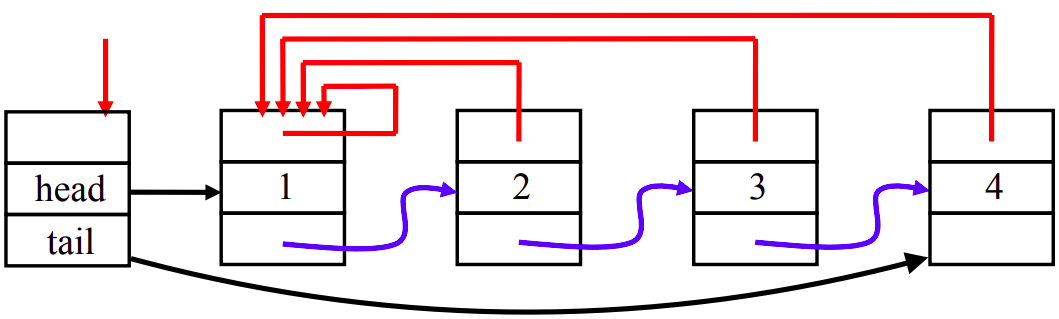
\includegraphics[width=0.8\textwidth]{merge-find-liste.png}
    \caption{\emph{Merge-find set} implementati come \emph{insiemi di liste}}
\end{figure}

\subsection{Implementazione basata su insiemi di alberi}
Ogni \emph{insieme} viene rappresentato da un \emph{albero} in cui ogni \emph{nodo}
contiene il proprio valore e un puntatore al \emph{padre}. La \emph{radice} è il
\emph{rappresentante} dell'\emph{insieme} e il puntatore al \emph{padre} punta
al \emph{nodo} stesso.

\begin{figure}[h!]
\centering
\begin{graph}
    \node[main] (1) {$1$};
    \node[main] (2) [below left of=1, xshift=5mm, yshift=-5.8mm] {$2$};
    \node[main] (3) [below right of=1, xshift=-5mm, yshift=-5.8mm] {$3$};
    \node[main] (4) [below of=2] {$4$};

    \path[->]   (1) edge[in=75, out=105, min distance=10mm] (1)
                (2) edge (1)
                (3) edge (1)
                (4) edge (2);

    \node[main] (5) [right of=1, xshift=20mm] {$5$};
    \node[main] (6) [below of=5] {$6$};
    \node[main] (7) [below of=6] {$7$};

    \path[->]   (5) edge[in=75, out=105, min distance=10mm] (5)
                (6) edge (5)
                (7) edge (6);
\end{graph}
\caption{\emph{Merge-find set} implementati come \emph{insiemi di alberi}}
\end{figure}

\noindent
In questo caso la \texttt{find} risale \emph{albero} fino alla \emph{radice} e
nel caso pessimo, questo costa $O(n)$. Per fare la \texttt{merge} invece, è
sufficiente cambiare il puntatore al \emph{padre} della \emph{radice} in uno
dei due \emph{alberi} in modo che punti all'altra \emph{radice}. Il costo, se
non consideriamo quello per la ricerca dei \emph{rappresentanti}, è $O(1)$.

\subsection{Implementazioni con tecniche euristiche}
Possiamo migliorare le implementazioni viste sfruttando qualche piccolo
accorgimento?

Nel caso dei \emph{merge-find set} basati su \emph{liste} potremmo provare ad
eseguire la \texttt{merge} modificando i puntatori della \emph{lista} più corta.
Per quanto riguarda gli \emph{alberi} invece, potremmo ridurre il costo della
\texttt{find} minimizzando l'\emph{altezza} degli \emph{alberi}. Tecniche di
questo tipo sono chiamate \emph{euristiche}, e gli algoritmi che le usano sono
detti \emph{euristici}.

\begin{definition}[Algoritmo euristico]
    È detto euristico un algoritmo progettato per risolvere un problema più
    velocemente, qualora i metodi tradizionali non siano sufficienti, oppure per
    ricavare una soluzione approssimata, qualora non sia possibile ricavarne una
    esatta.
\end{definition}

\paragraph{Euristica sul peso}
Approfondendo l'intuizione sulla lunghezza delle \emph{liste}, possiamo
memorizzare in ogni \emph{lista} l'informazione sulla propria lunghezza e
implementare la \texttt{merge} in modo che modifichi i puntatori dei \emph{nodi}
che stanno nella \emph{lista} più corta. La lunghezza può essere mantenuta in
$O(1)$ ed è possibile dimostrare che in questo tipo di implementazione il
\emph{costo ammortizzato} della \texttt{merge} si riduce ad $O(\log n)$.

\paragraph{Euristica sul rango}
Abbiamo detto che per gli \emph{alberi} conviene cercare di minimizzare le
\emph{altezze}, quindi associamo ad ogni \emph{nodo} $k$ il proprio
\emph{rango}, $rank[k]$, definito come segue:

\begin{definition}[Rango di un nodo]
    È definito rango di un nodo il numero di archi del più lungo cammino tra
    quel nodo e una delle proprie foglie.
\end{definition}
\begin{note}
    Possiamo anche definire il \emph{rango} di un \emph{nodo} come
    l'\emph{altezza} del \emph{sottoalbero} in esso radicato.
\end{note}

\noindent
A questo punto, per ridurre il costo della \texttt{find}, è sufficiente
modificare la \texttt{merge} in modo che, nel caso di \emph{alberi} con
\emph{ranghi} diversi, sia l'\emph{albero} con \emph{rango} minore ad essere
\q{agganciato} all'altro. In questa situazione, l'\emph{altezza}
dell'\emph{albero} con \emph{rango} maggiore non cambia, ma se invece i due
\emph{alberi} avessero pari \emph{rango}, l'\emph{altezza} finale andrebbe
incrementata di 1.

\begin{definition}[Legame tra il rango di un albero e il proprio numero di nodi]
    Un albero MFSET con radice $r$ e ottenuto tramite euristica sul rango ha
    almeno $2^{rank[r]}$ nodi.
\end{definition}
\begin{proof}[Dimostrazione]
    Procediamo per induzione sul \emph{rango} di $r$.

    \paragraph{Caso base: \bm{$rank[r]=0$}}
    Dopo l'inizializzazione della struttura ogni \emph{albero} ha $2^{rank[r]}
    =2^0=1$ \emph{nodi};

    \paragraph{Passo induttivo: \bm{$rank[r]>0$}}
    Facendo la \texttt{merge} di due \emph{alberi} $x$ e $y$ di \emph{rango}
    $rank[x]$ e $rank[y]$ distinguiamo due casi:
    \begin{enumerate}
        \item \bm{$rank[x]>rank[y]$}: il \emph{rango} dell'\emph{albero} $r$
        ottenuto è $rank[r]=rank[x]$. Per induzione, il numero di \emph{nodi} di
        $r$ è almeno pari a $2^{rank[x]}+2^{rank[y]}$ e quindi è maggiore di
        $2^{rank[x]}$;
        \item \bm{$rank[x]=rank[y]$}: il \emph{rango} dell'\emph{albero} $r$
        ottenuto è $rank[r]=rank[x]+1$. Per induzione, il numero di \emph{nodi}
        di $r$ è almeno pari a $2^{rank[x]}+2^{rank[y]}=2^{rank[x]}+2^{rank[x]}=
        2^{rank[x]+1}$;
    \end{enumerate}
\end{proof}

\noindent
Dal teorema appena dimostrato possiamo ricavare il seguente corollario:
\begin{definition}[Corollario]
    Un albero MFSET con radice $r$ e $n$ nodi ha un altezza minore o uguale di
    $\log n$.
\end{definition}
\begin{proof}[Dimostrazione]
    Vale la seguente relazione:
    \[n\geq 2^{rank[r]}\Leftrightarrow rank[r]\leq\log n\]
\end{proof}

\noindent
Detto questo, la \emph{complessità} della primitiva \texttt{find} è $O(\log n)$.

\paragraph{Euristica di compressione dei cammini}
Poiché il costo della \texttt{find} è legato all'\emph{altezza} degli
\emph{alberi}, se tutti avessero \emph{altezza} pari a $1$, cioè se il
\emph{padre} di ogni \emph{nodo} fosse la \emph{radice}, riusciremmo a ridurre
il costo di ogni invocazione a $O(1)$. Per raggiungere questo obiettivo possiamo
modificare l'implementazione della \texttt{find} in modo che, quando risaliamo
l'\emph{albero}, ogni \emph{nodo} modifichi il proprio puntatore al \emph{padre}
indicando il \emph{padre} del proprio \emph{padre}. In questo modo, la prima
invocazione di \texttt{find} costa $O(\log n)$, mentre ricerche successive
su \emph{nodi} già visitati costeranno $O(1)$.

\begin{figure}[h!]
    \centering
    \begin{graph}
        \node[main] (4a) {$4$};
        \node[main] (3a) [below left of=4a] {$3$};
        \node[main] (2a) [below left of=3a] {$2$};
        \node[main] (1a) [below left of=2a] {$1$};

        \path[->]   (1a) edge (2a)
                    (2a) edge (3a)
                    (3a) edge (4a)
                    (4a) edge[in=30, out=60, min distance=10mm] (4a);

        \node[]     (arrow) [below right of=3a, xshift=20mm]
        {$\xRightarrow{\texttt{\normalsize find(1)}}$};

        \node[main] (1b) [right of=arrow, xshift=20mm] {$1$};
        \node[main] (2b) [right of=1b] {$2$};
        \node[main] (3b) [right of=2b] {$3$};
        \node[main] (4b) [above of=2b] {$4$};

        \path[->]   (1b) edge (4b)
                    (2b) edge (4b)
                    (3b) edge (4b)
                    (4b) edge[in=75, out=105, min distance=10mm] (4b);
    \end{graph}
    \caption{Esempio di \emph{compressione dei cammini}}
\end{figure}

\begin{note}
    Applicando entrambe le \emph{euristiche}, il \emph{rango} non indica più
    l'\emph{altezza} del \emph{nodo}, bensì un limite superiore. Questo perché
    mantenere il valore corretto diventa troppo difficile (i.e. complesso) e
    comunque non è necessario.
\end{note}

\paragraph{Complessità}
Utilizzando entrambe le \emph{tecniche euristiche} viste, il \emph{costo
ammortizzato} di $m$ operazioni \texttt{merge-find} in un \emph{insieme} di $n$
elementi è $O(m\cdot\alpha(n))$, dove $\alpha(n)$ è la \emph{funzione inversa di
Ackermann} che ha una crescita estremamente lenta\footnotemark. Di conseguenza,
il \emph{costo ammortizzato} di una singola operazione è $O(1)$.

\footnotetext{Ad esempio, per $n\leq2^{65536}$, $\alpha(n)\leq5$}

\newpage
\paragraph{Implementazione}
\begin{code}{Merge-find set basati su insiemi di alberi}
\begin{minipage}[t]{0.48\textwidth}
\bc{int}[] parent\hfill\com{\emph{Vettore dei padri}}
\bc{int}[] rank\hfill\com{\emph{Ranghi} dei \emph{nodi}}

\ind\bc{MFSET} Mfset(\bc{int} n)\\
    \bc{MFSET} t = new \bc{MFSET}\\
    t.parent = new \bc{int}[1\dots n]\\
    t.rank = new \bc{int}[1\dots n]\\
    \indf for (i = 1 to n) do\\
        t.parent[i] = i\\
        t.rank[i] = 1\\
    \indf return t\\

\ind\bc{int} find(\bc{int} x)\\
    \indf if (parent[x] $\neq$ x) then\\
        parent[x] = find(parent[x])\\
    \indf return parent[x]\\
\end{minipage}
\hfill
\begin{minipage}[t]{0.48\textwidth}
    \ind merge(\bc{int} x, \bc{int} y)\\
        \bc{int} r$_x$ = find(x)\\
        \bc{int} r$_y$ = find(y)\\
        \indf if (r$_x$ $\neq$ r$_y$) then\\
            \indff if (rank[r$_x$] > rank[r$_y$]) then\\
                parent[r$_y$] = r$_x$\\
            \indff else\:if\:(rank[r$_y$]\;>\;rank[r$_x$])\:then\\
                parent[r$_x$] = r$_y$\\
            \indff else\\
                parent[r$_x$] = r$_y$\\
                rank[r$_y$] = rank[r$_y$] + 1\\
\end{minipage}
\end{code}

\subsection{Complessità}
Riassumendo, le \emph{complessità} delle possibili implementazioni dei
\emph{merge-find set} sono le seguenti\footnotemark:

\begin{table}[h!]
    \centering
    \renewcommand{\arraystretch}{1.2}
    \begin{tabular}{|p{0.33\textwidth}|c|c|}
        \hline
        \textbf{Algoritmo} & \texttt{find} & \texttt{merge}\\
        \hline
        Liste & $O(1)$ & $O(n)$\\
        \hline
        Alberi & $O(n)$ & $O(1)^+$\\
        \hline
        Liste con euristica sul peso & $O(1)$ & $O(\log n)^*$\\
        \hline
        Albero con euristica sul rango & $O(\log n)$ & $O(1)^+$\\
        \hline
        Albero con euristica sul rango e compressione dei cammini & $O(1)^*$ &
        $O(1)$\\
        \hline
    \end{tabular}
\end{table}

\footnotetext{
$\begin{aligned}[t]
    &*\text{: \emph{complessità ammortizzata};}\\
    &+\text{: Consideriamo solo il costo della \texttt{merge}, senza
    la ricerca dei \emph{rappresentanti} con la \texttt{find};}
\end{aligned}$
}